\documentclass[12pt, oneside]{article}
\usepackage[letterpaper, margin=1in]{geometry}
\usepackage[english]{babel}
\usepackage[utf8]{inputenc}
\usepackage{amsmath}
\usepackage{amsfonts}
\usepackage{amssymb}
\usepackage{tikz}
%\usepackage{tkz-fct}
\usepackage{pgfplots}
\pgfplotsset{width=10cm,compat=1.9}
\usepgfplotslibrary{statistics}
\usepackage{pgfplotstable}
%\usepackage{venndiagram}

\usepackage{fancyhdr}
\pagestyle{fancy}
\fancyhf{}
\rhead{\thepage \\Name: \hspace{1.5in}}
\lhead{BECA / Dr. Huson / 11.2 Algebra II\\* 27 April 2018 \\*\textbf{Classwork: Linear functions and graphing
}}

\renewcommand{\headrulewidth}{0pt}

\begin{document}


\subsection*{Solve equations}

Solve for the value of $x$.

\begin{enumerate}

\item   $12=x-5x$\\*[40pt]
\item   $\frac{1}{2}(5-x)=2x$\\*[60pt]
\item   $17=\frac{1}{2}x+4x-10$\\*[60pt]

\subsection*{Slope-intercept form}

What is the slope and $y$-intercept of each equation? 
\item   $y=3x-5$\\*[10pt]
\item   $6x+3y=9$\\*[40pt]


\subsection*{Function substitution}
\item Given $f(x)=3x+17$. Simplify $f(1)$.\\*[20pt]
\item Given $\displaystyle f(x)=-\frac{(2+4x)}{3}$. Simplify $f(-1)$.\\*[20pt]

\subsection*{Interpreting graphs}
Answer each question with as an ordered pair, in the form $(x, y)$.
\item In the graph shown, what point has the greatest $y$ value?\\*[30pt]
\item Name three points with the same $y$ value.\\*[30pt]
\item What is the $y$ value for $x=2$?\\*[30pt]
\item What is the $x$ value that would make $y=4$?\\*[30pt]
\item What is the value of $f(0)$?\\*[30pt]

\begin{figure}[!ht]
    \centering
    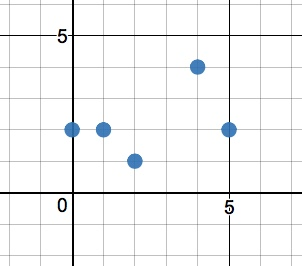
\includegraphics[width=0.35\textwidth]{discrete-domain-graph.jpeg}
\end{figure}

\newpage

\subsection*{Graphing linear functions}
Use pencil for graphs. Mark at least some of the values on each axis. Label each function with its name or equation. 
\item Graph the function $f(x)=\frac{1}{2}x+4$. 
\begin{enumerate}
    \item Write down the $y$-intercept.\\*[10pt]
    \item Write down the slope of $f(x)$.\\*[10pt]
    \item Mark the point $Q (6, 2)$.
    \item A second line, $g(x)$, is parallel to $f(x)$ and passes through point $Q$. Plot $g(x)$ on the graph.
    \item What is the $y$-intercept of $g(x)$?\\*[10pt]
\end{enumerate}

\begin{figure}[!ht]
    \centering
    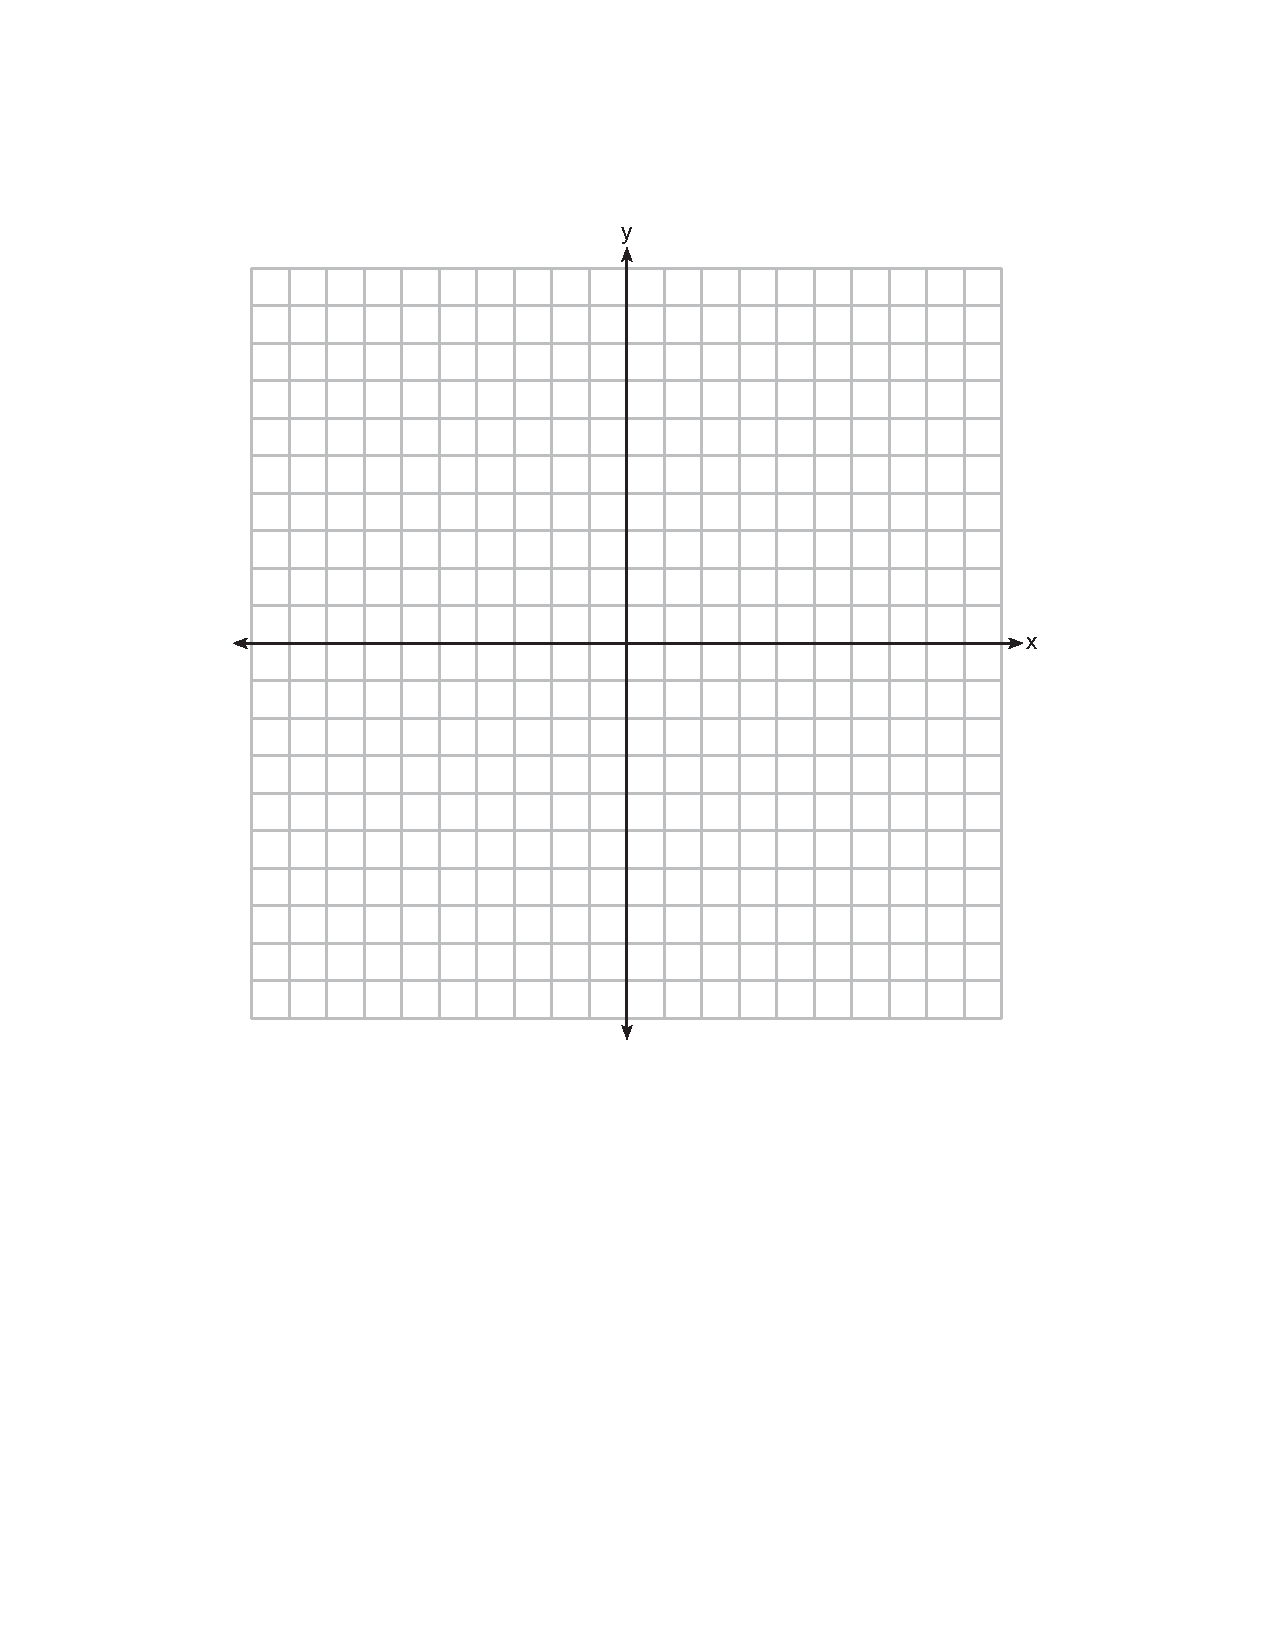
\includegraphics[width=0.75\textwidth]{regents-grid.pdf}
\end{figure}

\newpage
\item  
\begin{enumerate}
    \item Mark the point $P(3, -2)$ on the graph.
    \item The line $L_1$ has a $y$-intercept of 2 and passes through point $P$. Graph $L_1$.
    \item What is the slope of line $L_1$?\\*[20pt]
    \item What is the equation of line $L_1$?\\*[20pt]
    \item A second line, $L_2$ has the equation $x-y=-9$. Plot $L_2$ on the graph.
    \item What is the slope of $L_2$?\\*[30pt]
    \item Are the two lines $L_1$ and $L_2$ parallel, perpendicular, or neither?\\*[20pt]
    \item On the graph, mark the intersection of the two lines, the point $Q$, as an ordered pair.


\begin{figure}[!ht]
    \centering
    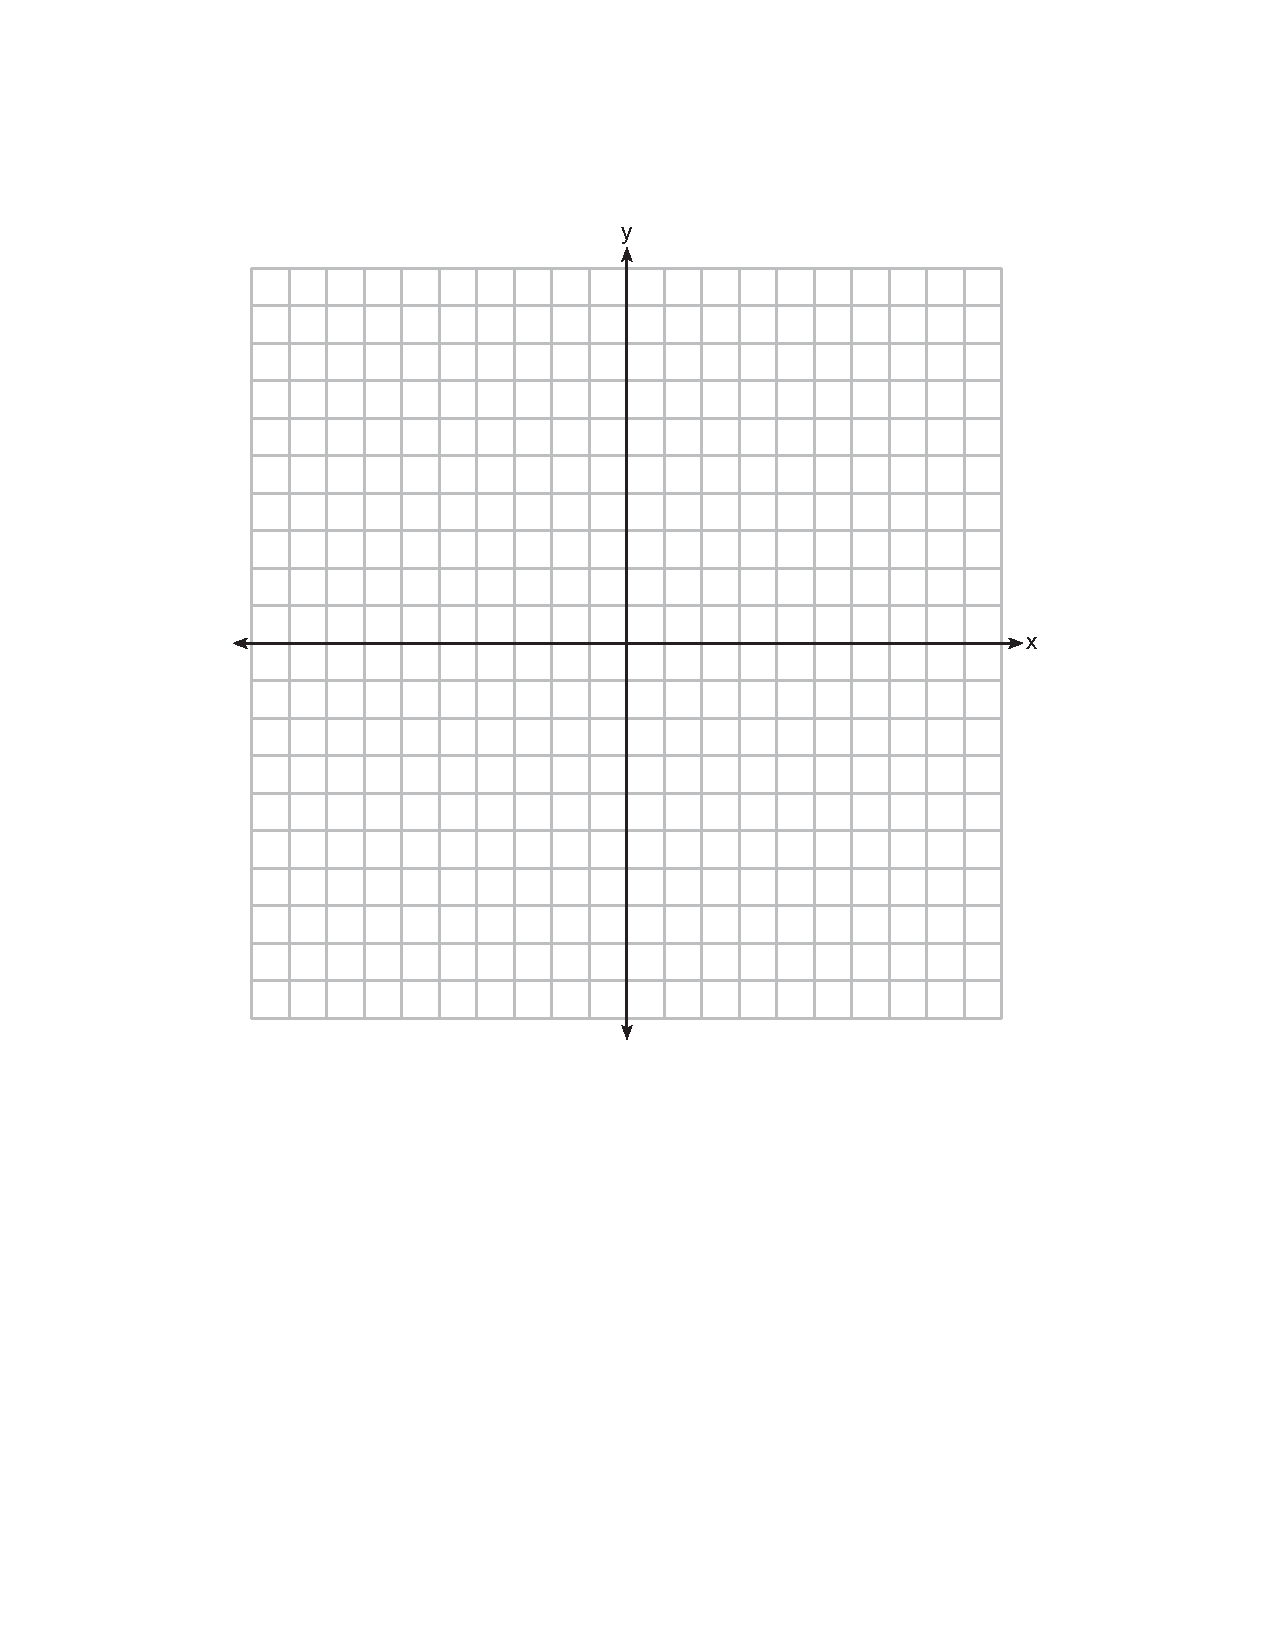
\includegraphics[width=0.65\textwidth]{regents-grid.pdf}
\end{figure}
\end{enumerate}


\end{enumerate}
\end{document}